\chapter{The Uniscale Frangi Filter} \label{ch:unifrangi}

	We now seek to harness the ideas introduced in \cref{ch:diffgeo} to the task at hand: identifying curvilinear content within images.

The Frangi filter, first described by Alejandro Frangi et al., is a widely used  Hessian-based filter
within image processing \cite{frangi-paper}. Hessian-based filters make use of the
logical ``proximity'' of the Hessian to notions of curvature of surfaces. Frangi's filter was orignally developed for vascular segmentation in images such as MRIs and it excels in that context \cite{frangi-paper}.
Several alternatively formulated Hessian-based filters exist \cite{sato-filter,lorenz-filter,olabarriaga-hessian-comparison}. These filters use information about the principal curvatures, approximated as eigenvalues of the Hessian, at each point in the image
to identify regions of significant curvature within an image.

We point out here that our image is of course a discrete structure and not a continuous surface, which was the object of concern in \cref{ch:diffgeo}.
In \cref{ch:scale-space-theory}, we will develop the notions of scale space, which will help us bridge the gap between continuous surfaces and discrete images. Using that approach, we shall consider the Frangi filter in its standard multiscale setting. For the time being, we continue to consider our images as continuous graphs, as the theory of the Frangi filter in its basic sense does not require the extra machinery of scale space theory.


The procedure for a continuous 2D image is as follows:
Let $\lambda_1, \lambda_2$ be the two eigenvalues of the Hessian of the image at point $(x, y)$,
ordered such that $\abs{\lambda_1} \leq \abs{\lambda_2}$, and define the Frangi vesselness measure for identifying bright curvilinear structures as %at scale $\sigma$ as:

\begin{equation} \label{eq:frangi-vesselness-measure}
\V(x,y) = \begin{cases}
0 & \text{if} \quad \lambda_2 > 0 \\
\exp\left\{-\frac{\Am^2}{2\beta^2}\right\}
\left(1 - \exp\left(-\frac{\Sm^2}{2c^2}\right)\right) & \text{otherwise}
\end{cases} \end{equation}
where
\begin{equation} \label{frangi-def-anisotropy-structureness}
\Am := \abs*{\frac{\lambda_1}{\lambda_2}}
\quad \textrm{and} \quad 
\Sm := \sqrt{\lambda_1^2 + \lambda_2^2}
\end{equation}
and $\beta$ and $c$ are tuning parameters. $\Am$ and $\Sm$ are known as the anisotropy measure and structureness measure, respectively. Similarly, we shall refer to the two factors in \cref{eq:frangi-vesselness-measure} as the anisotropy factor and structureness factor. We will also refer to $\lambda_2$ and $\lambda_1$ as the leading and trailing eigenvalues of the Hessian, respectively. Before we discuss appropriate values for $\beta$ and $c$, we first seek to highlight the significance of the two measures in \cref{frangi-def-anisotropy-structureness}.

\section{Anisotropy Measure} \label{sec:frangi.anisotropy}
The anisotropy (or directionality) measure $\Am$ is simply the ratio of magnitudes of $\lambda_1$ and $\lambda_2$. Since at a ridge point of a tubular structure, we should have $\lambda_1 \approx 0$ and $\abs*{\lambda_2} \gg \abs*{\lambda_1}$,
a very small value of $\Am$ would be present at a ridge of a tubular structure.
In \cref{fig:circular_trough_with_axes_vectors}, this situation is demonstrated. Here, $u_1$ and $u_2$ form the orthogonal set of Hessian eigenvectors with corresponding eigenvalues $\lambda_1$ and $\lambda_2$. At such a ridgelike structure, we could predict the largest change in curvature to be straight down the ridge (in the direction of $u_2$), and the direction of least curvature to be directly along the ridge (in the direction  of $u_1$). The leading eigenvalue $\lambda_2$ should be large and negative, and $\lambda_1$ should be approximately zero.

\begin{figure} \centering
  \includegraphics[width=0.8\linewidth]{circular_trough_with_axes_vectors}
  \caption{The principal eigenvectors at a ridge-like structure} 
  \label{fig:circular_trough_with_axes_vectors}
\end{figure}. 


Of course, if the the ridge is perfectly circular along its cross section, as in \cref{sec:calculate-weinmap-of-a-ridge}, we note that the leading  $\lambda_1$ would likewise be 0 at any such point.  One could also imagine a similar situation in which the dropoff from crest to bottom gets increasingly steep. In such a case, $\lambda_2$ as a function of transverse position would in fact be largest nearest to the bottom. This thought experiment should dispel a na\"{i}ve misunderstanding of the power of a Frangi filter: a high anisotropy measure (and a large structureness measure \vcleanup{define structureness first}) will not in general identify the crests of a ridge-like structure--it only will highlight that such a pixel is on a ridge-like structure at all. In fact, the particular leading eigenvalue calculated in \cref{sec:calculate-weinmap-of-a-ridge} actually increases as $x$ moves farther away from the crest. In general, the anisotropy measure will not necessarily be at a maximum at the crest of the ridge, but instead, somewhere along it.

Similiarly, the vessel we we wish to identify can not be reasonably expected to behave as perfectly as our toy example. There will likely be small aberrations in a ridgelike structure, such as small divots or depressions in an overall ridge-like structure. Of importance in our data set later (\cref{sec:NCS-data-set}), there will be points where we seem to "lose" our ridgelike structure,
but this is simply due to an error in the sample.

Importantly, this formulation does not require $\lambda_1$ to be approximately zero, just that the curvature in the downward direction is much more significant than in the transverse direction.

Also the crest could be really flat (``hangar shaped''), in which case both are around zero. At the crest of the ridge, we would actually expect both $u_1$ and $u_2$ to be around 0, whereas a point somewhere between the crest and the ``foot'' of the ridge to contain the maximum $u_2$. We will fix this issue specifically by casting this as a multiscale problem in \cref{ch:multifrangi}.

Two other ideas that could fix some other discrepancies mentioned above is to identify these ridges on their own, or also where the 'feet are'. We will discuss these ideas in \cref{ch:segmentation}.

\section{Structureness Measure} \label{sec:frangi-structureness}

There is another concern with using the pure ratio $\Am:= \abs{\lambda_1 / \lambda_2}$ as an identifying feature of ridgelike structures apart from the ones listed above. We could have $\abs*{\lambda_2} \gg \abs*{\lambda_1}$ in a relative sense, but still have $\lambda_2 \approx 0$. As a rather extreme example, we should certainly wish to differentiate a point on the surface where $\lambda_2 \approx 10^{-5} $ and $\lambda_1 \approx 10^{-10}$ from another point where $\lambda_2 \approx 10000$ and $\lambda_2 = 0.1$.

A natural fix to differentiate these points is to introduce a ``structureness'' measure to insure that there is in fact significant curvilinear activity at the point in question. Frangi used $\Sm:= \sqrt{(\lambda_1)^2 + (\lambda_2)^2}$, which is in fact the Frobenius norm of the Hessian matrix. Inclusion of the structureness factor with an appropriately chosen parameter $c$ should result in a high vesselness measure only for regions of significant curvilinear content.


\section{The Frangi Vesselness Measure}

Our goal then is to attach a numerical measure to each pixel in the image %(at a particular scale $\sigma$)
that is large when the anisotropy measure $\Am$ and the structureness measure $\Sm$ is sufficiently large.

The form Frangi arrived at in \cref{eq:frangi-vesselness-measure} in which a factor of $\exp(\cdots)$ and $(1 - \exp(\cdots))$ are multiplied together are simply to ensure that the final vesselness measure $\V$ is largest when $\Am$ is small and $\Sm$ is large enough, with rapid decay in other situations.

Frangi further strengthened the filter by adding an additional case to \cref{eq:frangi-vesselness-measure}, ensuring that $\lambda_2$ is not positive. If we are indeed at a curvilinear ridge, then it is a critical point, and we need the second derivative of the surface in the maximal direction to be negative, which hasn't been accounted for as yet in our formulation of $\Am$ and $\Sm$ -- we wish (for our purposes) to only identify when we are finding crests. $\Am$ will still be small and $\Sm$ will still be large however if we identify a ``trough''.

The only perceivable difference is that the maximum normal curvature will be positive--we are at a local minimum in the direction of $u_2$. In situations where we wish to only identify ridges (bright curvilinear structures), we simply exclude all points where there is not a negative curvature in the maximal direction. Conversely, we could only seek to find valleys (dark curvilinear structures) and thus require $\lambda_2 > 0$, and set the vesselness measure to zero when $\lambda_2 < 0$.



\section{Choosing Parameters $\beta$ and $c$}

The parameters $\beta$ and $c$ are meant to scale so that the peaks of the anisotropy factor $\exp(\frac{-\Am^2}{2\beta^2})$ and the structureness factor $(1-\exp\left(\frac{-\Sm^2}{2c^2}\right))$ coincide enough to be statistically significant at highly curvilinear structures, but rapidly decay in areas not associated with curvilinear content. What values of these parameters are appropriate is ultimately dependent on the context of the problem.

For the default value of the structureness parameter $c$, Frangi suggested that half of (the Frobenius norm of the) Hessian matrix is appropriate, simply because the minimum value of $\Sm$ is zero, and its maximum value is exactly the maximum value of the Frobenius norm over the surface.

With this in mind we would like to introduce the scaling factor $\gamma$, so that $ c = \gamma \Smax$. This creates a minor annoyance though: although the anisotropy factor can certainly attain a value of 1, if $c$ is to take this suggested value, the maximum value of the structureness factor is somewhat smaller than 1. In fact,
\begin{equation}
\begin{aligned}
\max\{\V \} &\le \max\left(
\exp\left(\frac{-\Am^2}{2\beta^2}\right)
\right)
\max\left(
\left(1 - \exp\left(\frac{-\Sm^2}{2(\gamma \Smax)^2}\right)\right)
\right) \\
&\le \max\left\{
\left(1 - \exp\left(\frac{-\Sm^2}{2(\gamma \Smax)^2}\right)\right)
\right\} \\
&= 
\left(1 - \exp\left(\frac{-(\Smax)^2}{2(\gamma \Smax)^2}\right)
\right)
= \left(1 - \exp\left(\frac{-1}{2\gamma^2}\right)
\right)
\end{aligned}
\end{equation}

Thus, when $\gamma$ takes the suggested value of $\gamma = 1/2$, the above calculation suggests that
the maximum theoretical value that the Frangi filter could attain for any image is
$ \max \{ \V \} \le 1 - \exp\left( -1 \right) \approx .8647$.
This (among other obvious reasons) certainly justifies Frangi's description of the vesselness measure as only ``probability-like.'' Still, we would like the filter's sensitivity to relative structureness to not have the effect of dampening the Filter as a whole, so we will introduce a rescaling factor $a_\gamma$, which is a explicit function of $\gamma$ that rescales $\V$ so that the structureness factor has a maximum value of 1 regardless of choice of $\gamma$. Our modified Frangi vesselness measure is thus

%    \begin{minipage}{\textwidth} \centering
\begin{gather} \label{eq:V_rescaled}
\V(x_0,y_0) = \begin{cases}
0 & \text{if} \quad \lambda_2 > 0 \\
a_\gamma \exp\left(\frac{-\Am^2}{2\beta^2}\right)
\left(1 - \exp\left(\frac{-\Sm^2}{2(\gamma \Smax)^2}\right)\right) & \text{otherwise}
\end{cases} \\
\shortintertext{where, as before,}
%\begin{equation} \label{frangi-def-anisotropy-structureness-v1}
\Am := \abs*{\frac{\lambda_1}{\lambda_2}}
\;,\;
\Sm := \sqrt{\lambda_1^2 + \lambda_2^2}
\;\textrm{and}\;
a_\gamma = \left(1-\exp\left(\frac{-1}{2\gamma^2}\right)\right)^{-1} \notag\\
%\end{equation}
\shortintertext{and}
%\begin{equation*}
\abs*{\lambda_1} \le \abs*{\lambda_2}
\; \textrm{are eigenvalues of the Hessian matrix at point} \; (x_0, y_0).
%\end{equation*}
\end{gather}
%    \end{minipage}

For $\beta$, Frangi suggested an innocuous intermediate point, $\beta=1/2$ (and thus $2\beta^2 = 1/2$).
As we will show later, choosing the structureness parameter $\gamma$ is rather important for the context especially if the background (non-ridgelike structure) is significant and noisy. $\beta$ should be strengthened/relaxed depending on how dramatic the curvilinear structures are in comparison to the rest of the image. We shall show empirically that contexts in which more 'bloblike' structures are known to be present than that for which the Frangi filter was originally designed, we will benefit from a smaller choice of $\beta$.

Considering as the anisotropy measure $\abs*{\lambda_1 / \lambda_2} \in [0,1]$,  we can actually visualize how much the 
anisotropy factor varies depending on our choice of $\beta$, as seen in \cref{fig:anisotropy-parameter-demo}.

We can theoretically choose any values $0 < \beta, \gamma < \infty$ for the two parameters. Two particular limits are of theoretical interest.

As $\beta \to \infty$, the anisotropy factor tends to $1$, and the Frangi filter will simply return the value of the structureness factor. Similarly, as $\gamma$ tends to $0$, the structureness factor tends to $1$, and the Frangi filter will return the value of the anisotropy factor. We will use this fact in \cref{ch:results-analysis} to provide a visual demonstration of each individual factor. The limits in the other directions are less interesting; if either $\beta \to 0$ or $\gamma \to \infty$, their respective factors will tend to $0$, making the entire filter zero everywhere.

\begin{figure}[t] \centering
  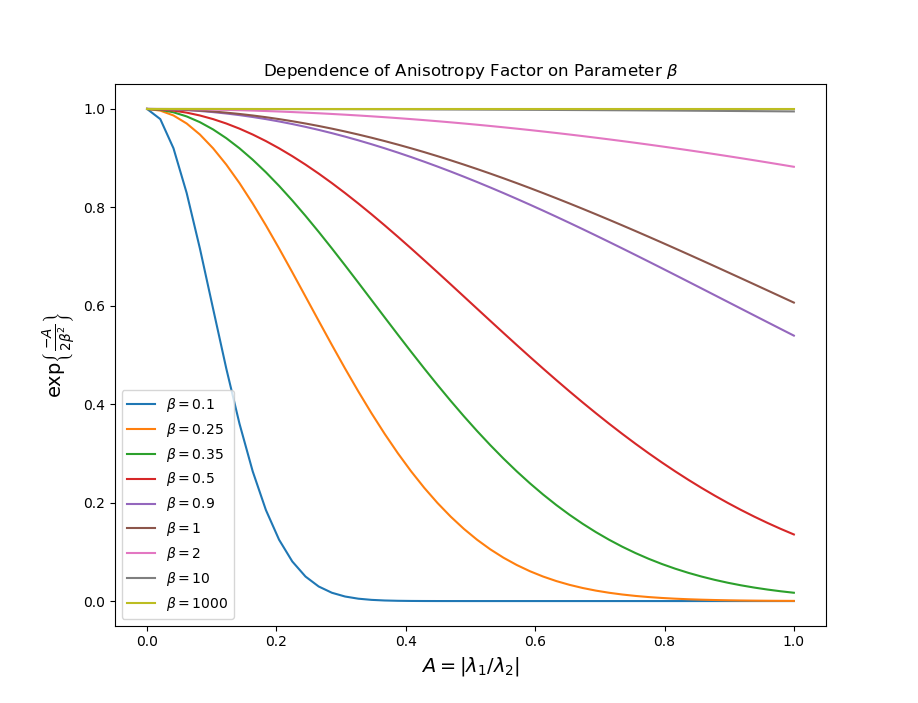
\includegraphics[height=0.4\textheight]{anisotropy_parameter_demo}
  \caption{Dependence of the anisotropy factor on its parameter}
  \label{fig:anisotropy-parameter-demo}
\end{figure}

\begin{figure}[t] \centering
  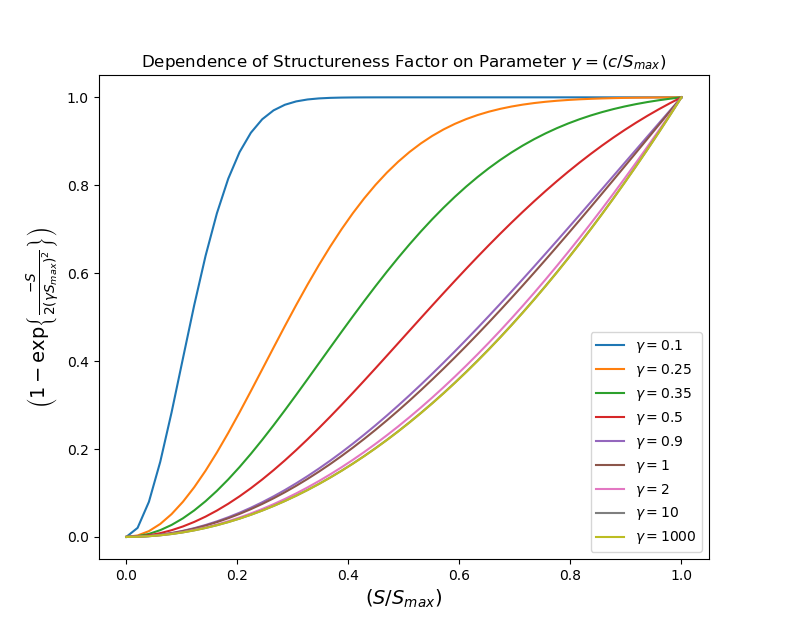
\includegraphics[height=0.4\textheight]{structureness_parameter_demo}
  \caption{Dependence of the structureness factor on its parameter}
  \label{fig:structureness-parameter-demo}
\end{figure}

\cref{fig:structureness-parameter-demo} is a similar presentation of the dependence of the structureness kernel on its parameter $\gamma$.
A convenient by-product of our redefinition of $\gamma$ actually is that can group together $\Sm$ with the $\Smax$ that appears in the denominator, allowing us to refer to a structureness ratio $\Sm/\Smax$. In fact, we could perfectly well define the Frangi filter to be in terms of this ratio--though we refrain presently since we acknowledge specific cases where $c$ can be chosen to be fixed independent of a calculated $\Smax$ value.


The ultimate choice of these parameters $\beta$ and $\gamma$ have the overall effect of tuning the selectivity of the Frangi filter itself. In \cref{fig:frangi3d-selection}, we show the shape of our rescaled filter depends on the anisotropy measure $\abs{\lambda_1 / \lambda_2}$ and the ``structureness ratio'' $\Sm/\Smax$ for some illustrative choices of $\beta$ and $\gamma$. Each of these filters has been rescaled with $a_\gamma$. The steepness of the first figure suggests that the filter is in fact, stricter compared to the default parameter selection. \cref{subfig:frangi3d-loose} shows the filters continued strength over a much larger range of values, indicating that it may not work effectively. In particular, choosing $\gamma$, and thus $c$, poorly will lead to quite a lot of noise.
An interesting manifestation of this is that the default implementation of the Frangi filter \cite{scipy} chooses an seemingly arbitrarily fixed value for the structureness parameter, perhaps causing many na\"ive applications of the Frangi filter to give a needlessly poor result, simply becuase the filter was not correctly parametrized in relation to the image at hand.

\begin{figure}[t] \centering
\subfloat[Strict]{\includegraphics[height=0.3\textheight]{4-rs}} \label{subfig:frangi3d-strict} \\
\subfloat[Standard]{\includegraphics[height=0.3\textheight]{14-rs}} \label{subfig:frangi3d-default} \\
\subfloat[Loose $\gamma$]{\includegraphics[height=0.3\textheight]{12-rs}} \label{subfig:frangi3d-loose} \\
\caption{Strictness of Frangi filter based on parametrization}
\label{fig:frangi3d-selection}
\end{figure}

	We now take a quick tangent from our description of the Frangi filter to develop and justify our ``multiscale'' approach.
	
